% Template for ICASSP-2019 paper; to be used with:
%          spconf.sty  - ICASSP/ICIP LaTeX style file, and
%          IEEEbib.bst - IEEE bibliography style file.
% --------------------------------------------------------------------------
\documentclass{article}
\usepackage{spconf,amsmath,amssymb,graphicx,todonotes}
\usepackage{url}
\usepackage{booktabs}
\usepackage{algorithm}
\usepackage{algpseudocode}
\usepackage{epstopdf}
% Example definitions.
% --------------------
\def\x{{\mathbf x}}
\def\L{{\cal L}}
\def\lone{{$l^1$}}
\def\ltwo{{$l^2$}}
\def \fatR {{ \mathbb R}}
\DeclareMathOperator{\Tr}{Tr}
\providecommand{\norm}[1]{\lVert#1\rVert}
\newtheorem{problem1}{\noindent \textbf{Problem}}
\newtheorem{theorem}{\noindent \textbf{Theorem}}
\newtheorem{algorithm1}{\noindent \textbf{Algorithm}}
\newtheorem{lemma}{\noindent \textbf{Lemma}}
\newtheorem{conjecture}{\noindent \textbf{Conjecture}}

%\makeatletter
%\DeclareRobustCommand\onedot{\futurelet\@let@token\@onedot}
%\newcommand{\onedot}{\futurelet\@let@token\@onedot}
%\def\@onedot{\ifx\@let@token.\else.\null\fi\xspace}

\def\eg{\emph{e.g.\ }}
\def\Eg{\emph{E.g.\ }}
\def\ie{\emph{i.e.\ }}
\def\Ie{\emph{I.e.\ }}
\def\cf{\emph{c.f.\ }} 
\def\Cf{\emph{C.f.\ }}
\def\etc{\emph{etc.\ }} 
\def\vs{\emph{vs.\ }}
\def\wrt{w.r.t.\ }
 \def\dof{d.o.f.\ }
\def\etal{\emph{et al.\ }}
\def\Win{W_{\text{in}}}
\def\Wout{W_{\text{out}}}


%\renewcommand{\todo}[1]{{\color{red}\textbf{#1}}}
%\makeatother


\newcommand{\tworowtab}[2]{\begin{tabular}{cc|} #1 \\ #2\relax\end{tabular}}
\newcommand{\threerowtab}[3]{\begin{tabular}{ccc|} #1 \\ #2 \\ #3\relax\end{tabular}}



% Title.
% ------
\title{Robust Self-Calibration of Constant Offset Time-Difference-of-Arrival}
%
% Single address.
% ---------------
%\name{Kenneth Batstone$^1$, Gabrielle Flood$^1$, Thejasvi Beleyur$^1$, Viktor Larsson$^1$, Magnus Oskarsson$^1$, Holger R.\ Goerlitz$^3$, Kalle {\AA}str{\"o}m$^1$)\thanks{Thanks to WASP, ELLIIT, SSF m m.}}
%\address{Centre for Mathematical Sciences, Lund University, Sweden}
%\name{Kenneth Batstone, Gabrielle Flood, Viktor Larsson, Magnus Oskarsson, Kalle {\AA}str{\"o}m)\thanks{Thanks to WASP, ELLIIT, SSF m m.}}
%\address{Centre for Mathematical Sciences, Lund University, Sweden}
%\name{Kenneth Batstone\textsuperscript{1}, Gabrielle Flood\textsuperscript{1}, Thejasvi Beleyur\textsuperscript{3}, Viktor Larsson\textsuperscript{2}, 
%Holger R.\ Goerlitz\textsuperscript{3}, Magnus Oskarsson\textsuperscript{1}, Kalle {\AA}str{\"o}m\textsuperscript{1} \thanks{Thanks to WASP, ELLIIT, SSF m m.}}
\name{K.\ Batstone\textsuperscript{1}, G.\ Flood\textsuperscript{1}, T.\ Beleyur\textsuperscript{3}, V.\ Larsson\textsuperscript{2}, 
H.\ R.\ Goerlitz\textsuperscript{3}, M.\ Oskarsson\textsuperscript{1}, K.\ {\AA}str{\"o}m\textsuperscript{1} \thanks{This work was partially supported by the following funding bodies: strategic research projects ELLIIT and eSSENCE, The Sten K. Johnson foundation, Swedish Foundation for Strategic Research
project - Semantic Mapping and Visual Navigation for
Smart Robots - (grant no. RIT15-0038), Wallenberg Artificial
Intelligence, Autonomous Systems and Software Program
(WASP) funded by Knut and Alice Wallenberg Foundation, Emmy Noether research (grant no. GO2029/2-1) of the 
Deutsche Forschungsgemeinschaft to HRG.}}
\address{\tworowtab{Centre for Mathematical Sciences}{Lund University, Sweden\textsuperscript{1}}
\tworowtab{Dept.\ of Computer Science}{ETH Zurich, Switzerland\textsuperscript{2}}
%\tworowtab{Acoustic and Functional Ecology}{Max Planck Inst.\ for Ornithology, Seewiesen, Germany\textsuperscript{3}}}
\threerowtab{Acoustic and Functional Ecology}{Max Planck Inst.\ for Ornithology}{Seewiesen, Germany\textsuperscript{3}}}
%\address{\threerowtab{Centre for Mathematical Sciences}{Lund University, Sweden\textsuperscript{1}}
%\threerowtab{Department of Computer Science}{ETH Zurich, Switzerland\textsuperscript{2}}
%\threerowtab{Department of Computer Science}{ETH Zurich, Switzerland\textsuperscript{3}}}

% tbeleyur@orn.mpg.de
% Thejasvi Beleyur,
%
% For example:
% ------------
%\address{School\\
%	Department\\
%	Address}
%
% Two addresses (uncomment and modify for two-address case).
% ----------------------------------------------------------
%\twoauthors
%  {A. Author-one, B. Author-two\sthanks{Thanks to XYZ agency for funding.}}
%	{School A-B\\
%	Department A-B\\
%	Address A-B}
%  {C. Author-three, D. Author-four\sthanks{The fourth author performed the work
%	while at ...}}
%	{School C-D\\
%	Department C-D\\
%	Address C-D}
%
\begin{document}
%\ninept
%
\maketitle
%
\begin{abstract}
In this paper we study the problem of estimating receiver and sender positions  from time-difference-of-arrival measurements, assuming an unknown constant time-difference-of-arrival offset. This problem is relevant for example for repetitive sound events. In this paper it is shown that there are three minimal cases to the problem. One of these (the five receiver, five sender problem) is of particular importance. A fast solver (with run-time under $4~ \mu s$) is given. We show how this solver can be used in robust estimation algorithms, based on RANSAC, for obtaining an initial estimate followed by local optimization using a robust error norm. The system is verified on both real and synthetic data. 
\end{abstract}
%
\begin{keywords}
Time-difference-of-arrival, Constant Offset, RANSAC, Minimal Problem
\end{keywords}
%
\vspace{-5pt}
\section{Introduction}
\label{sec:intro}
\vspace{-5pt}
%\todo[inline]{Short intro. What is the problem}

The problem of estimating receiver-sender node positions from measured arrival times of radio or sound signals is a key issue in different applications such as microphone array calibration, radio antenna array calibration, mapping and positioning. This field is well researched but in this paper we will focus on the anchor-free sensor network calibration both in terms of time-of-arrival measurements (TOA) and time-difference-of-arrival measurements (TDOA). 
For time-of-arrival the planar case of three receivers and three senders (3R/3S) was solved in \cite{stewenius-phd-2005}.
For the full 3D case the over-determined problem (10R/4S) was studied in \cite{pollefeys-nister-icassp-08}, where a solver for this non-minimal case was provided.   
There are actually three minimal cases for the 3D case, namely (4R/6S), (5R/5S) and (6R/5S). A practical solver was presented in
\cite{kuang-burgess-etal-icassp-13}. There are in general $38$, $42$ and $38$ solutions respectively for the three different set ups. 
Faster solvers for these minimal cases were provided in \cite{larsson2017polynomial}.

%Far-field approximation:
% \cite{Thrun05c} 
%  \cite{kuang-ask-etal-icpram-12}.  
  
% RANSAC \cite{fischler-bolles-ca-81}, 
%  \cite{eckart-young-1936}. 
%   \cite{wiberg-1976} 
   
% Missing data - robustness: 
% \cite{aanaes-etal-pami-2002,buchanan-cvpr-2005,ke-kanade-cvpr-2005,eriksson-hengel-pami-2012}.  
% 
% \cite{candes-etal-acm-2009,garg2013dense,olsson-oskarsson-scia-2011} 
% 
%  \cite{cabral-et-al-iccv-2013}. 
%A few recent works \cite{mackey2011divide,larsson-olsson-etal-eccv-14} 
%
% in~\cite{jiang-cvpr-2015}. 

%\todo[inline]{Contributions of the paper}

In this paper we study the constant offset TDOA self-calibration problem. It is a problem that naturally arises e.g.\ when signals are emitted  with a known period. As an estimation problem it lies between TOA and full TDOA. In the paper we study the minimal (5R/5S) problem and provide a fast (few $\mu s$) solver. 
Robust parameter estimation often use the hypothesize and test paradigm, e.g.\ using random sampling consensus, \cite{fischler-bolles-ca-81} or one of its many variants \cite{chum2003locally,raguram2013usac,korman2018latent}. In these frameworks minimal solvers are important building blocks for generating model hypotheses, and 
%DEGSAC - degenerate ransac solver - relevant if we do 4x4 solver 
we show in the  paper how a minimal solver can be used for robust parameter estimation of sender positions, receiver positions and unknown offset. 
The system is capable of handling missing data, outliers and noise. The algorithms are tested on synthetic data as well as real data,  
in an office environment and in a cave.
%RANSAC using the minimal solver. Analysis of RANSAC behaviour on random data. 
%
%Robust system - detect outliers, find initial estimate for parameters, followed by non-linear optimization for ML estimate. 
%
%Evaluation on real and synthetic data. (Comparison to other methods).
The methods are straightforward to generalize for degenerate configurations which arise if senders or receivers are restricted to a plane or to a line. %\todo{VL: I don't think we should mention rank 1,2 here, since reader probably does not know about the rank constraints yet.}
 
\vspace{-5pt}
\section{Time-difference-of-arrival self~calibration}
\label{sec:todoa}
\vspace{-5pt}
The problem we are considering involves $m$ receiver positions  $\mathbf{r}_i \in \fatR^3$, $ i = 1, \dots, m,$ and  
$n$ sender positions $\mathbf{s}_j \in \fatR^3$, $ j = 1, \dots, n$.
This could for example represent the microphone positions and locations of sound emissions, respectively.  
Assume that the arrival time of a sound $j$ to receiver $i$ is $t_{ij}$ and that the time that sound $j$ is emitted is $T_j$. 
Multiplying the travel time $t_{ij} - T_j$ with the speed $v$ of the signal we obtain the distance between senders and receiver,
\begin{equation}
v (t_{ij}-T_j)   = {\norm{\mathbf{r}_i - \mathbf{s}_j}}_2 ,
\label{eq:tdoa}
\end{equation} 
where  ${\norm{.}}_2$ is the \ltwo-norm. The speed $v$ is throughout the paper assumed to be  known and constant. 

In many settings the times of emissions $T_j$ are unknown, but regular, \eg
\begin{equation}
T_j = k_1 j + k_0, 
\label{eq:regular}
\end{equation}
where the interval $k_1$ is known. Inserting \eqref{eq:regular} into \eqref{eq:tdoa} we
obtain 
\begin{equation}
v (t_{ij}-k_1 j - k_0)   = {\norm{\mathbf{r}_i - \mathbf{s}_j}}_2 . 
\end{equation}
Assuming an erroneous (but regular) emission time 
$\tilde{T}_j = k_1 j + \tilde{k}_0$ and 
introducing (the measured) $z_{ij} = v (t_{ij}-\tilde{T}_j)$ and (the unknown) $o = v (k_0-\tilde{k}_0)$ yields the following expression
\begin{equation}
 z_{ij}   = {\norm{\mathbf{r}_i - \mathbf{s}_j}}_2 + o. 
\end{equation}
Note that this is a simplified variant of the general time-difference-of-arrival problem (see \eg  \cite{kuang2013stratified}), which allows for a different offset $o$ for every $j$, 
\begin{equation}
 z_{ij}   = {\norm{\mathbf{r}_i - \mathbf{s}_j}}_2 + o_j.
\end{equation} 

\noindent \begin{problem1} \label{prob_misstoa}
({{Constant Offset Time-Difference-of-Arrival  Self-Calibration}}) Given measurements $\tilde{z}_{ij}$ 
\vspace{-5pt}
\begin{equation}
\tilde{z}_{ij} = {\norm{\mathbf{r}_i - \mathbf{s}_j}}_2 + o  + \epsilon_{ij}, 
\label{eq:distance}
\vspace{-5pt}
\end{equation}
for a subset $W \subset I$ of all the receiver-sender index pairs $I = \{ (i,j) | i = 1, \ldots m, j = 1, \ldots, n \}$ determine receiver positions $\mathbf{r}_i$, $ i = 1, \dots, m$ and sender positions $\mathbf{s}_j$,  $j = 1, \dots, n$ and offset $o$. 
Here the errors $\epsilon_{ij}$ are assumed to be either 
{\bf inliers}, in which case the errors are small ($\epsilon_{ij} \in N(0,\sigma)$) or {\bf outliers}, in which case the measurements are way off. 
\end{problem1}
Here we will use the set $\Win$ for the indices $(i,j)$ corresponding to the inlier measurements and $\Wout$ for the indices corresponding to the outlier set. 
\vspace{-5pt}
\section{Local optimization and the low~rank~relaxation}
\label{sec:rank}
\vspace{-5pt}
If an initial estimate of the parameters $\theta_1 = \{ R, S, o \}$ is given and if the set of inliers is known, then refinement of the estimate can be found by optimization methods, \eg Levenberg-Marquardt (LM) \cite{levenberg1944method,marquardt1963algorithm}, 
\begin{equation}
\min_{\theta_1} f(\theta_1) = \sum_{(i,j) \in \Win} (z_{ij} - ( {\norm{\mathbf{r}_i - \mathbf{s}_j}}_2 +o) )^2 .
\end{equation}

There is an interesting relaxation to the problem, that exploits the fact that the matrix with elements $ (z_{ij}-o)^2 $ is rank $5$, \cite{pollefeys-nister-icassp-08}. Further simplifications use the double compaction method \cite{kuang2013stratified}. The double compaction matrix $M$ is defined as the matrix with elements
\begin{equation}
M_{ij}=(z_{ij}-o)^2 -a_i-b_j,
\label{eq:dc}
\end{equation}
 and it can be shown to have rank $3$, i.e.\ $M = U^T V$, where $U$ is of size $3 \times m$ and $V$ is of size $3 \times n$. 
The relaxed problem involves a set of parameters
$\theta_2 = \{ U, V, b, a, o \}$. Here the constraints can be written as
\begin{equation}
z_{ij} =  \sqrt{u_i^T v_j + a_i + b_j} + o ,
\end{equation}
where $u_i$ denotes column $i$ of $U$ and $v_j$ denotes column $j$ of $V$.
Refinement of parameters can be done by performing local optimization on 
\begin{equation}
\min_{\theta_2} f(\theta_2) = \sum_{(i,j) \in \Win} \left ( z_{ij} - ( \sqrt{u_i^T v_j + a_i + b_j} + o ) \right )^2 .
\label{eq:relaxed}
\end{equation}

\vspace{-5pt}
\section{Minimal problems and solvers}
\label{sec:minimal}
\vspace{-5pt}
By counting equations and unknowns, one finds that there are three minimal problems. The first two are the symmetric case when $m=4, n=7$ or $m=7, n=4$. This case is not addressed in this paper, but we believe it to be difficult to solve. The other case is $m=n= 5$. Here, we first present a solver for the constant offset and then discuss how to solve for sender and receiver positions. 

%{\bf Minimal solver for $o$:}

Given a $5 \times 5$ matrix, $Z$, with time-difference-of-arrival measurements $z_{ij}$, the rank $3$ constraint on the double compaction matrix in \eqref{eq:dc} 
can be written as
\begin{equation}
f(o) = \det ( C^T (Z-o)^{\circ 2} C )  = 0, 
\end{equation}
where
\begin{equation}
C = \begin{pmatrix}
-1 & -1 & -1 & -1\\
1 & 0 & 0 & 0\\
0  & 1 & 0 & 0\\
0 & 0 & 1 & 0 \\
0 & 0 & 0 & 1 
\end{pmatrix} 
\end{equation}
and $^{\circ 2}$ denotes element-wise squaring (Hadamard power).
Although the elements of $ (Z-o)^{\circ 2}$ are of degree 2 in $o$, the quadratic terms cancel out after multiplication with $C^T$ and $C$. Thus the elements of $C^T (Z-o)^{\circ 2} C$ are linear in $o$.
Since the determinant is linear in each column, the determinant $f(o)$ is a polynomial of degree four in the offset $o$. This can be summarized as 
\begin{theorem}
Given time-difference-of-arrival measurements from five receivers to five senders, there are four possible offsets $o$, given as the roots to the fourth degree polynomial $f(o)$, counting complex roots and multiplicity of roots. 
\end{theorem}
 
%\begin{equation}
%\begin{pmatrix}
%-1 & 1 & 0 & 0 & 0\\
%-1 & 0 & 1 & 0 & 0\\
%-1 & 0 & 0 & 1 & 0\\
%-1 & 0 & 0 & 0 & 1
%\end{pmatrix}
%\begin{pmatrix}
%z_{11}-0 & z_{12}-0 & z_{13}-0 & z_{14}-0 & z_{15}-0 \\
%z_{21}-0 & z_{22}-0 & z_{23}-0 & z_{24}-0 & z_{25}-0 \\
%z_{31}-0 & z_{32}-0 & z_{33}-0 & z_{34}-0 & z_{35}-0 \\
%z_{41}-0 & z_{42}-0 & z_{43}-0 & z_{44}-0 & z_{45}-0 \\
%z_{51}-0 & z_{52}-0 & z_{53}-0 & z_{54}-0 & z_{55}-0 
%\end{pmatrix}
%\begin{pmatrix}
%-1 & -1 & -1 & -1\\
%1 & 0 & 1 & 0\\
%0  & 1 & 0 & 0\\
%0 & 0 & 1 & 0 \\
%0 & 0 & 0 & 1 
%\end{pmatrix}
%)  = 0
%\end{equation}

For each solution $o$ it is possible to generate a solution $\theta_2$ to the relaxed problem, 
according to 
%\begin{align}
%b =& \begin{pmatrix} (z_{11} \! - \! o)^2  \! \!  &  \! \!  (z_{12}-o)^2  \! \!  &  \! \!  (z_{13}-o)^2 \! \!  &  \! \!   (z_{14}-o)^2 \! \!  &  \! \!   (z_{15}-o)^2 \end{pmatrix}, \\
%a = & \begin{pmatrix} 0 \\ (z_{21}-o)^2 -(z_{11}-o)^2\\ (z_{31}-o)^2 -(z_{11}-o)^2 \\ (z_{41}-o)^2 -(z_{11}-o)^2 \\ (z_{51}-o)^2 -(z_{11}-o)^2 \end{pmatrix},\\ 
%U = & \begin{pmatrix} 0 & u_2 & u_3 & u_4 & u_5\end{pmatrix},  \\
%V = & \begin{pmatrix}0 & v_2 & v_3 & v_4 & v_5\end{pmatrix} ,
%\end{align} 
\begin{equation*}
\! b \! = \! \begin{pmatrix} (z_{11} \! - \! o)^2  \! \!  &  \! \!  (z_{12}-o)^2  \! \!  &  \! \!  (z_{13}-o)^2 \! \!  &  \! \!   (z_{14}-o)^2 \! \!  &  \! \!   (z_{15}-o)^2 \end{pmatrix} \! ,
\end{equation*}
\begin{equation}
a =  \begin{pmatrix} 0 \\ (z_{21}-o)^2 -(z_{11}-o)^2\\ (z_{31}-o)^2 -(z_{11}-o)^2 \\ (z_{41}-o)^2 -(z_{11}-o)^2 \\ (z_{51}-o)^2 -(z_{11}-o)^2 \end{pmatrix},
\end{equation}
\begin{equation}
U =  \begin{pmatrix} 0 & u_2 & u_3 & u_4 & u_5\end{pmatrix}, 
\end{equation}
\begin{equation}
V =  \begin{pmatrix}0 & v_2 & v_3 & v_4 & v_5\end{pmatrix} ,
\end{equation}
where $\begin{pmatrix}u_2 & u_3 & u_4 & u_5\end{pmatrix}^T  \begin{pmatrix} v_2 & v_3 & v_4 & v_5\end{pmatrix}$ is any rank $3$ factorization of the matrix $C^T (Z-o)^{\circ 2} C$. 

From a solution $\theta_2$ to the relaxed problem it is possible to upgrade to a solution $\theta_1$ to the original problem. This involves solving a system of polynomial equations. The procedure was first described in \cite{kuang-burgess-etal-icassp-13}, where an algorithm for solving this was presented. Recently, a faster algorithm was presented in \cite{larsson2017polynomial}.

An efficient implementation for calculating the four solutions of the offset $o$ given the measurements $z$ takes $4~ \mu s$ for a C++-implementation. Generating the solution $\theta_2$ to the relaxed problem adds a few $\mu s$. However, calculating a solution $\theta_1$ to the original problem takes another $22 ~ms$. Thus, it is advantageous to estimate the parameters of the relaxed problem and postpone the upgrade from $\theta_2$ to $\theta_1$ as a final step, see Table~\ref{Tabletime}.
%Discuss speed of solvers. Argue that it might be useful to only estimate o, since this solver is so fast. 

\begin{table}
\caption{Execution times for $5 \times 5$ minimal solvers steps. Notice that the steps of calculating $o$ and the relaxed solution is significantly faster than upgrading to the full solution}
\centering
\vspace{4mm}
\begin{tabular}{@{}ccc@{}} \toprule
%& \multicolumn{5}{c}{CS (dB)} & \multicolumn{5}{c}{SSIM} \\ \cmidrule(r){2-11}
Implementation & Matlab  & C++ \\
\midrule 
Calculation of $o$ & $38 \, \mu s$ & $3.7 \, \mu s$ \\
Calculation of $\theta_2 = \{ U,V,a,b,o \}$ & $100 \, \mu s$ & N/A \\
Calculation of $\theta_1 = \{ R,S,o \}$ & $600 \, ms$ & $22 \, ms$ \\
\bottomrule
\end{tabular}
\label{Tabletime}
\end{table}

\vspace{-5pt}
\section{Using RANSAC for five rows}
\label{sec:ransac}
\vspace{-5pt}
We propose the use of the fast minimal solver in an hypothesize and test framework to obtain (i) a initial estimate on the offset $o$ and (ii) an initial inlier set.  The steps are described in Algorithm~\ref{a_offset}
%This is done as follows. 
%\begin{algorithm1}
%\begin{enumerate}
%\item Select $5$ random rows. Select $5$ random columns. Find the four solutions on $o$ given the time-difference-of-arrival measurements. 
%\item For each solution $o$, calculate the relaxed solution $\theta_2 = (U,V,a,b)$.
%\item For selected rows and for each remaining column, check for inliers according to xxx
%\end{enumerate}
%\end{algorithm1}
\begin{algorithm}
\caption{Offset RANSAC}\label{a_offset}
\begin{algorithmic}[1]
%\State Select $5$ random rows. Select $5$ random columns. Find the four solutions on $o$ given the time-difference-of-arrival measurements. 
\State Randomly select $5$ rows and columns. Find the four solutions on $o$ given the time-difference-of-arrival measurements. 
\State For each solution $o$, calculate the relaxed solution $\theta_2 = \{ U,V,a,b,o \}$.
\State For selected rows and for each remaining column, check for inliers according to the residuals in \eqref{eq:relaxed}.
\end{algorithmic}
\end{algorithm}







%There are two key questions here. First, how many inliers do we expect for the null hypothesis, \ie if all data is random noise. Secondly, how many iterations do we typically need to find all the inliers, when the data is 
\vspace{-5pt}
\section{Robust estimation of parameters}
\label{sec:ransac}
\vspace{-5pt}
We use these minimal solvers with RANSAC as described in the previous section to find one or several initial estimates of the parameters $\theta_2$ for a subset of five receivers and $k$ senders. The solution is extended to additional rows and/or columns using robust techniques as described in \cite{batstone2016robust}. During this process it is useful to keep the errors down by occasionally refining the solutions using local optimization. This has shown to reduce failures, see e.g.\ \cite{engels-stewenius-etal-06,klein2007parallel}.
In the proposed estimation algorithm we postpone the upgrade from $\theta_2$ to $\theta_1$ until we have found a good solution involving a large portion of the receiver and sender positions. 
\vspace{-5pt}
\section{Experimental Validation}
\label{sec:exp}
\vspace{-5pt}
\subsection{Minimal Solver}
\vspace{-5pt}

To test the numerical accuracy and robustness of our minimal solver we conducted an experiment using simulated data without noise. We generated a large number of instance problems (10,000) with known offsets. We then ran our solvers and compared the returned solutions with the ground truth solution. For each instance problem we recorded the distance to the closest solution. In Figure~\ref{fig:f_hist} the resulting histogram of the logarithm of the absolute errors are shown. As can be seen, both implementations get close to machine precision. 
\begin{figure}
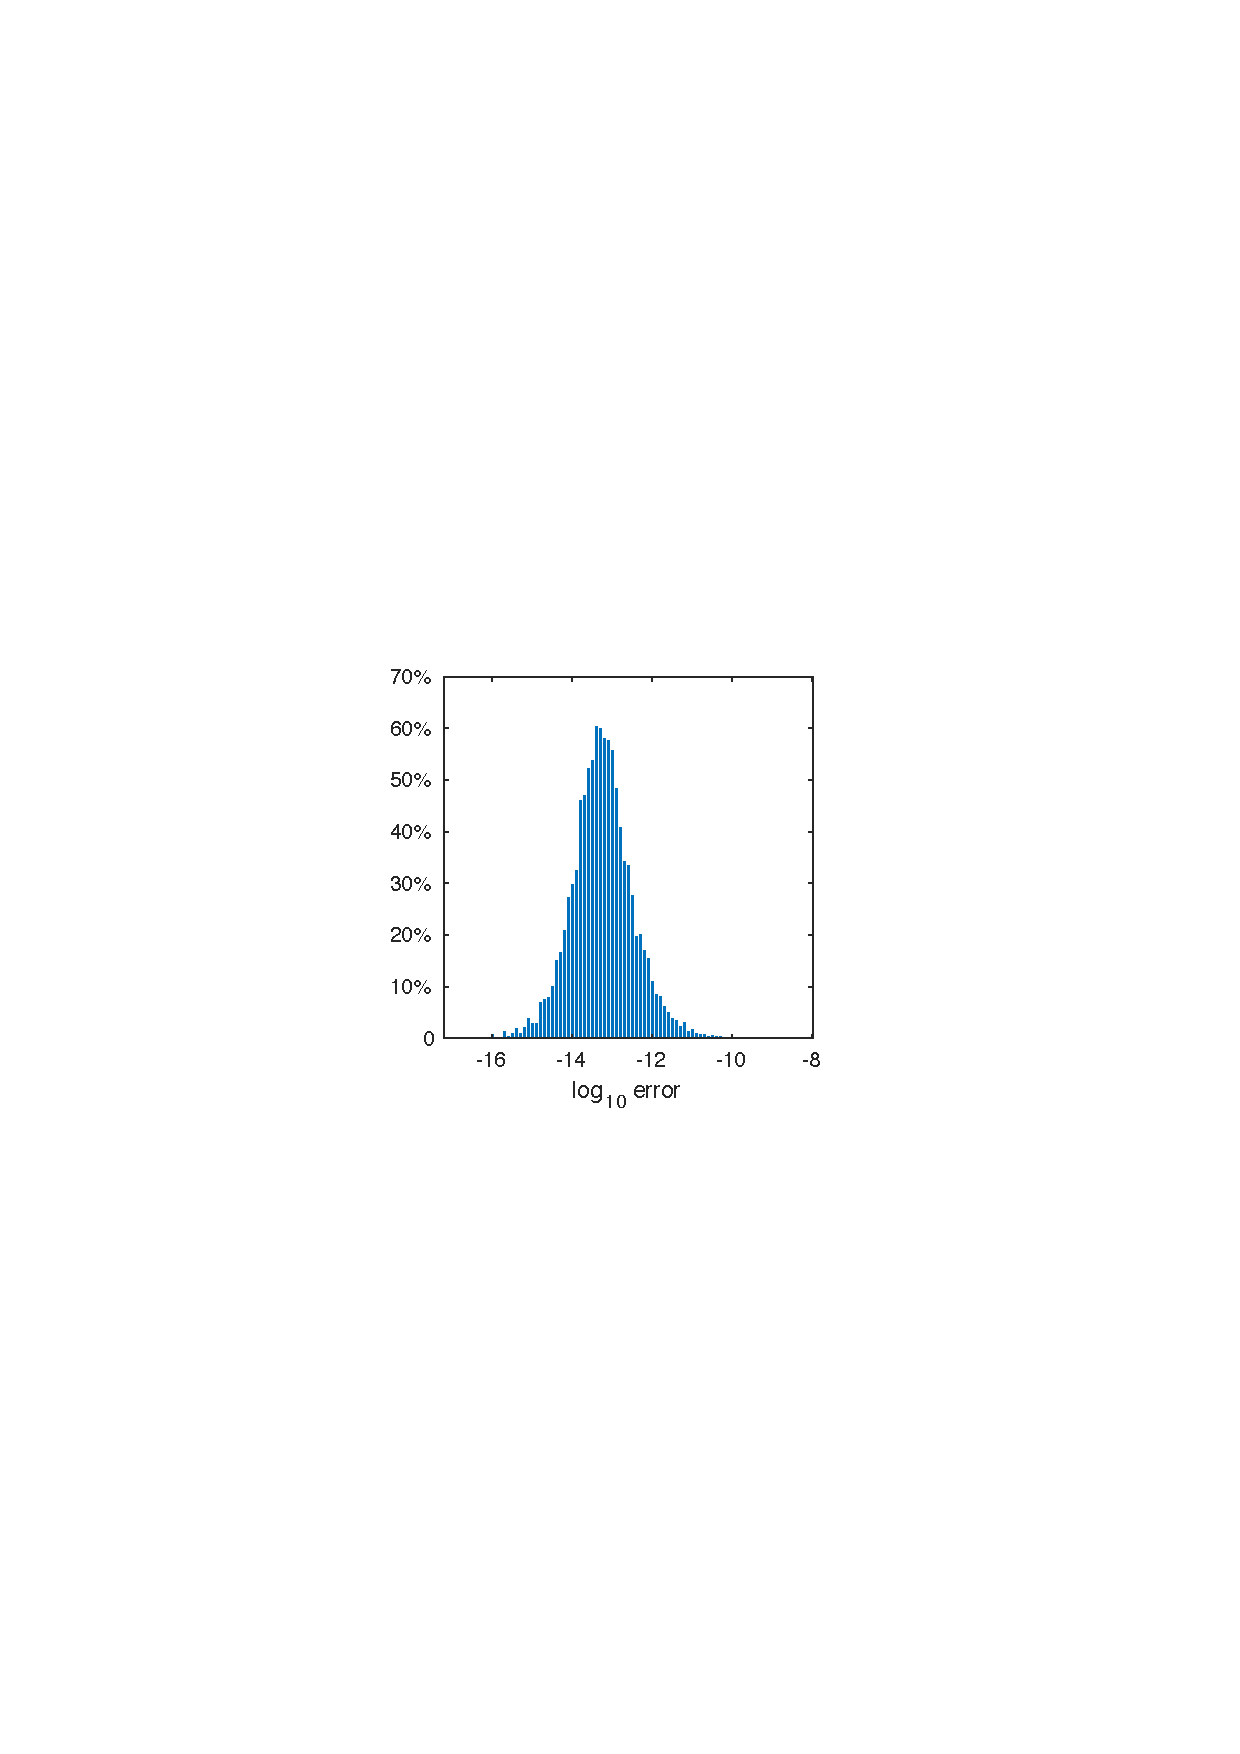
\includegraphics[width=0.23\textwidth]{figs/hist_matlabsolver.pdf}
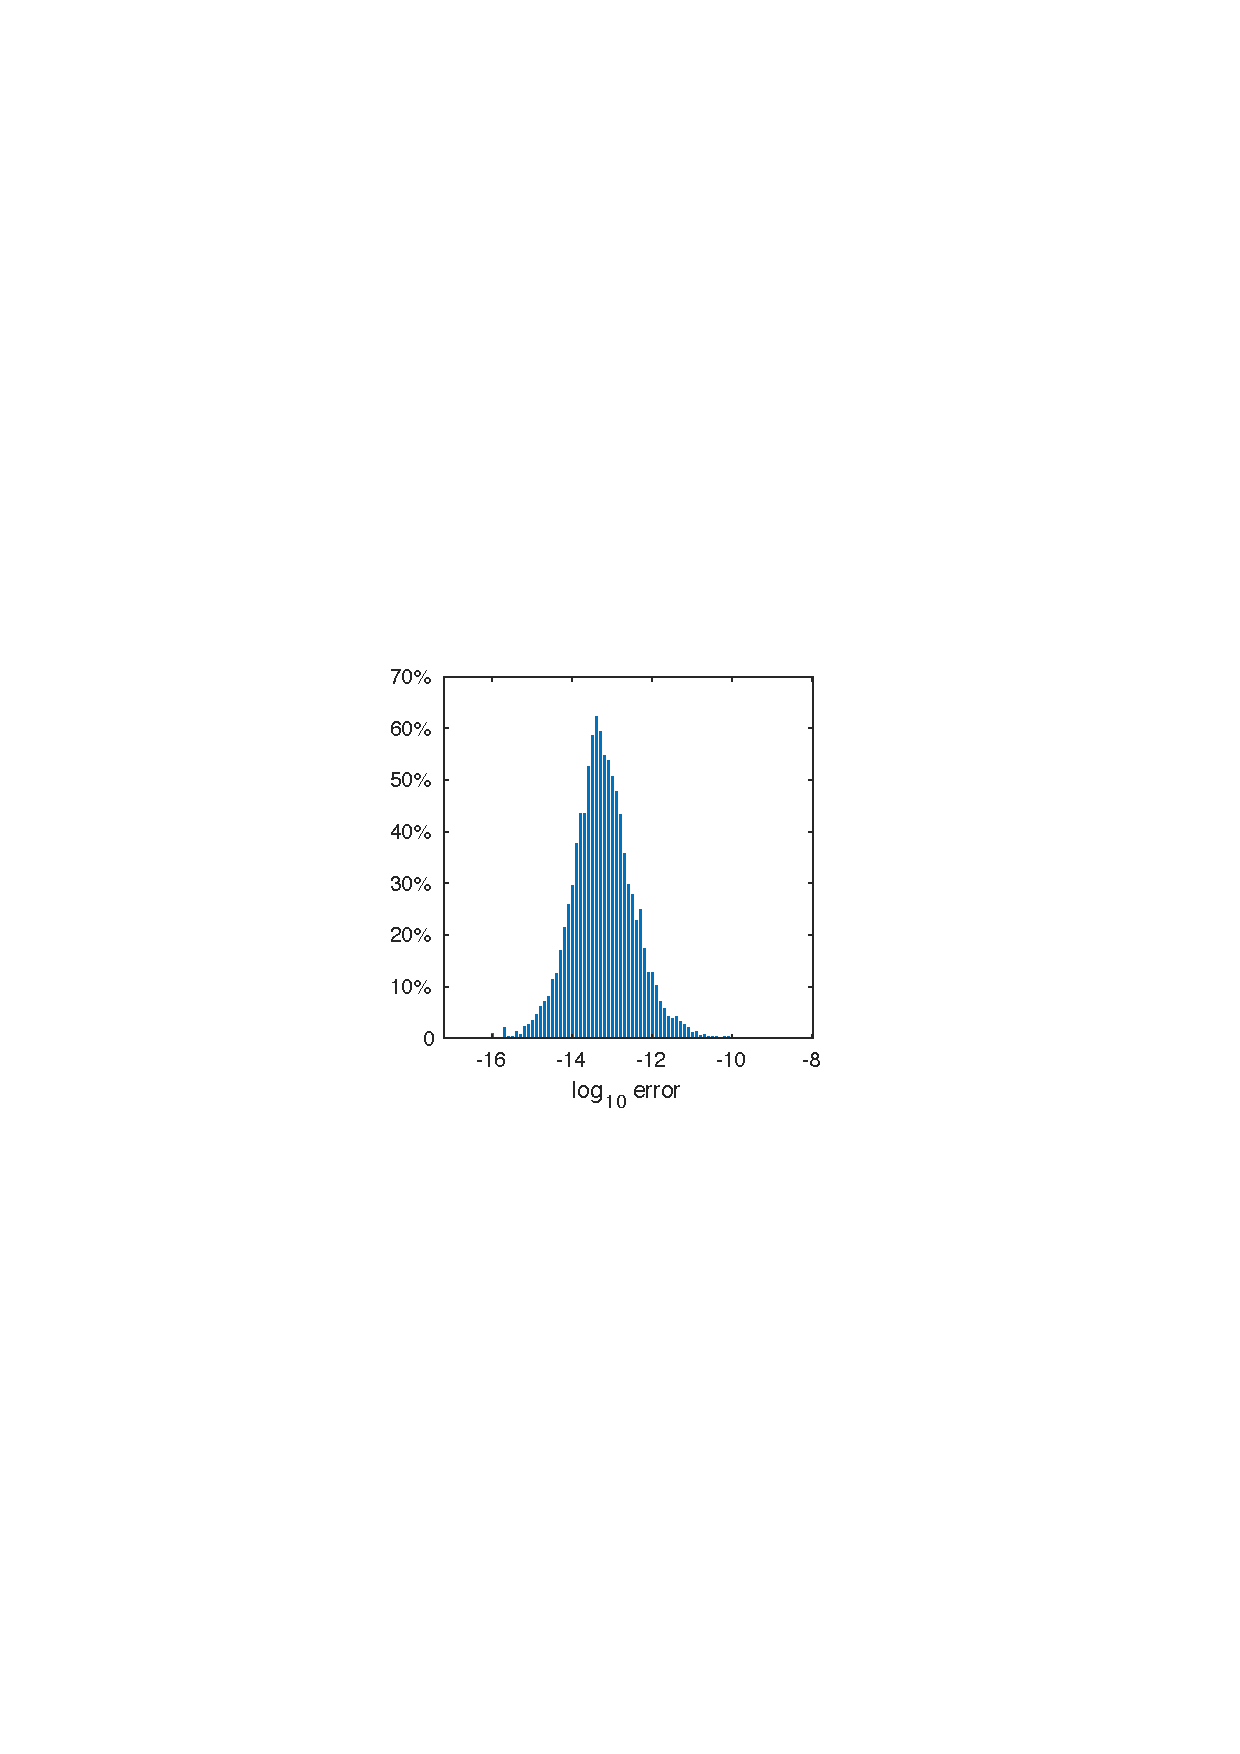
\includegraphics[width=0.23\textwidth]{figs/hist_mexsolver.pdf}
\caption{Left shows the histogram of the logarithm of the absolute errors, for the Matlab implementation of our minimal solver. To the right the corresponding histogram for the C++ implementation.}
\label{fig:f_hist}
\end{figure}






%\subsection{RANSAC for 5 receivers and $n$ senders}
%
%In order to understand how many inliers to expect, when using pure noise, i.e.\ if the data consists of outliers only, we generate matrices of 
%size $5 \times n$ where each element is drawn for a uniform distribution in the interval $[0,1]$. In Fig.~\ref{f_random_ransac_hists}
%the histogram of the number of inliers is shown for ransac thresholds $0.05$, $0.1$ and $0.2$ for random $5 \times 100$ matrices. Since the
%random elements are uniform $0-1$, we expect high number of inliers if thresholds become as large as $1$. The distributions are somewhat similar to binomial distributions. A reasonable simplification is to study the mean and standard deviation of these distributions. 
%In Fig.~\ref{f_mean_std_100} the mean and standard deviation is shown as a function of thresholds $T$ for random $5 \times 100$ matrices. 
%
%
% resulting histogram of the logarithm of the absolute errors is shown. To the left is the result of the solver implemented 
%
%
%%\begin{figure}
%%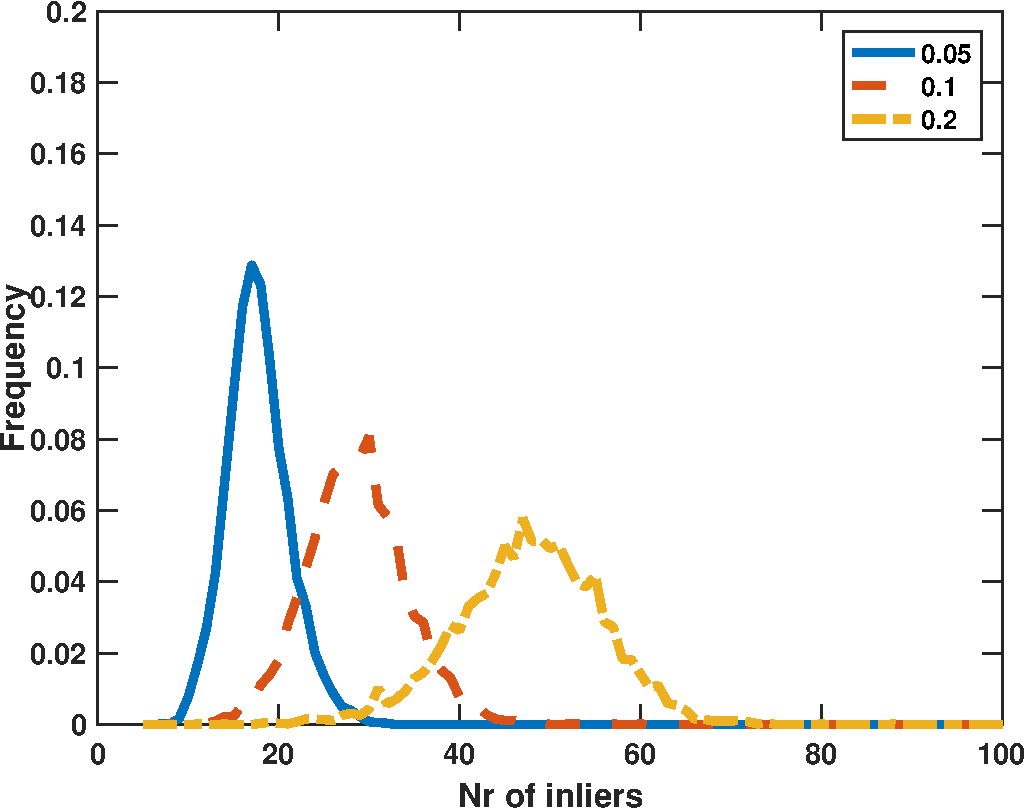
\includegraphics[width=0.23\textwidth]{figs/InlierHistograms.pdf}
%%\caption{Estimated probability functions of the number of inliers for random $5 \times 100$ matrices using three different thresholds $T$.}
%%\label{f_random_ransac_hists}
%%\end{figure}
%
%%\begin{figure}
%%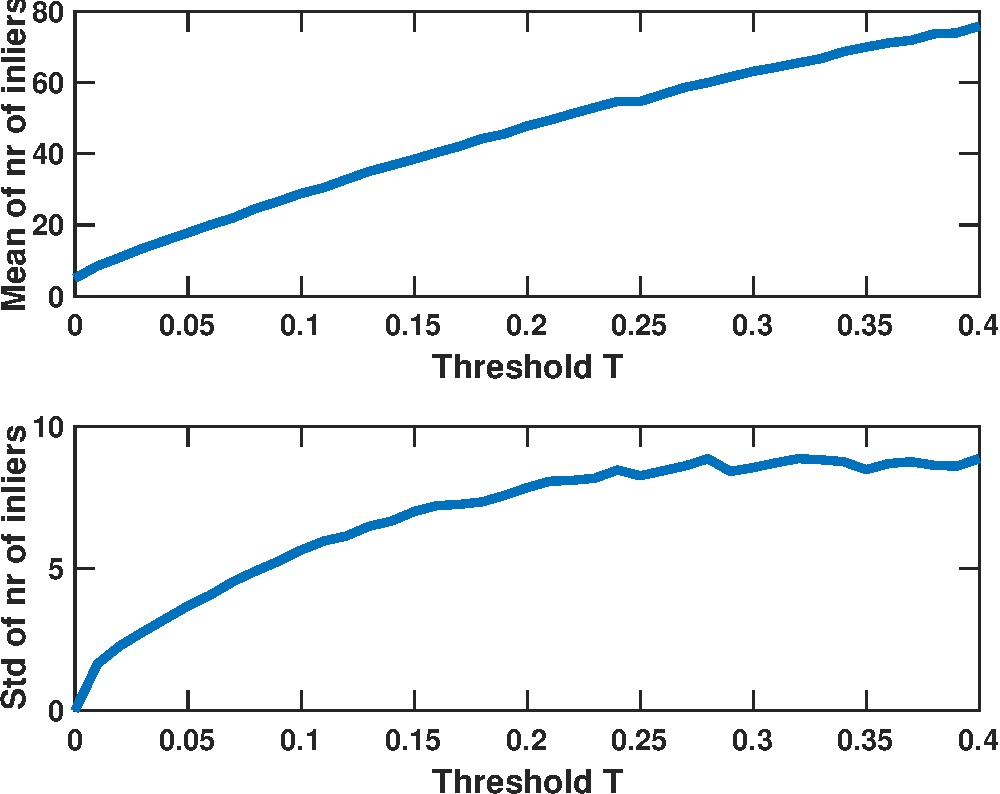
\includegraphics[width=0.43\textwidth]{figs/MeanStdInliers.pdf}
%%\caption{Mean and standard deviation of the number of inliers as a function of the threshold $T$, for random $5 \times 100$ matrices. }
%%\label{f_random_mean_std}
%%\end{figure}
%
%\begin{figure}
%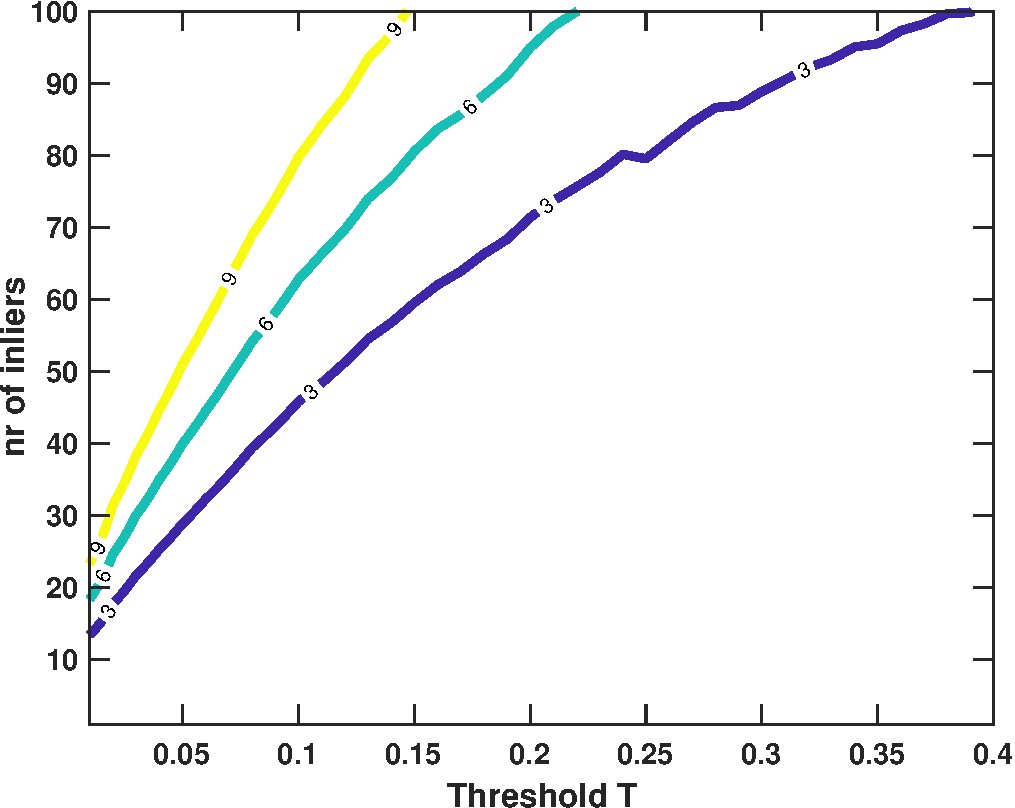
\includegraphics[width=0.43\textwidth]{figs/Significance.pdf}
%\caption{Significance xxx. }
%\label{f_random_significance}
%\end{figure}
%
%
%
%
%Study how many inliers one gets on random data. Figure. 
%Discussions on how many iterations are needed. 
%If the number our outliers is small, a good solutions with a high number of inliers can be found quickly. Few iterations. 

%\subsection{Synthetic data}
%???
\vspace{-5pt}
\subsection{Experimental Setup for Real Data}
\vspace{-5pt}
We have tested our system on (i) experiments made in an office environment and (ii) experiments made at the Orlova Chuka cave, Bulgaria. 

For the office experiments, 12 microphones (8x t.bone MM-1, 4x Shure SV100) were positioned around a room ($\sim 3 \times 5~m^2$) and measured using a laser to obtain ground truth positions of the microphones with an error of $\pm 2~ mm$. The space was cleared of most the furniture to create an open space to conduct the experiment in. The sound recordings were captured using a Roland UA-1610 Sound Capture audio interface and automatically amplified. The recordings were made using the open source software Audacity 2.3.0 with a sampling frequency of $96~kHz$ on a laptop. A synthetically generated chirp was then played using a simple loudspeaker every half second for $30~s$ while moving the speaker around in the room. 

For the cave experiments, 12 microphones (4x Sanken CO-100K, 8x Knowles SPU0410) were positioned in a section of the cave, four microphones were placed on an inverted T array near one wall, while the other eight microphones were placed on the adjacent wall. The sound recordings were captured using pre-amplifiers (Quadmic, RME) and two synchronised Fireface 800 (RME) audio interfaces running at a sampling frequency of $192 ~kHz$. Recording and playback were controlled via a custom written script based on the sound device library
%(Geier, 2015) 
\cite{geier2015}
in Python 2.7.12 
%(Van Rossum & Drake Jr, 1995)
\cite{van1995python}.
Ultrasonic chirps ($8~ms$, $16-96~kHz$ upward hyperbolic sweep) were played every second via one of the audio interfaces, amplified (Basetech AP-2100) and presented through a Peerless XT25SC90-04 loudspeaker. The speaker was attached to a 3-m-long pole and slowly waved in the approximately $5 \times 9 \times 3 ~m^3$ recording volume. Playbacks were done past 6:00 am to prevent disturbing the resident bat population.
\vspace{-5pt}
\subsection{Experimental Evaluation for Real Data}
\vspace{-5pt}
Once the office recordings were taken, an algorithm was used to find the chirps in the captured sound recordings and the algorithm then outputs the $z_{ij}$ matrix.  This can then be used in our RANSAC scheme, Algorithm~\ref{a_offset}. For this experiment we used the (5R/5S)  minimal solver. A fixed number of iterations was used; 100 iterations for the initial selection of 5 receivers and senders, then the extension to more columns and rows was allowed until there was no better solution. The tolerance was set to $T=0.01$ for the initial selection and extension of rows and column.

Once the initial values have been estimated, it underwent $l^{2}$ optimization on the inlier set. The results of the estimated microphone positions after the optimization are shown in Figure~\ref{f_454H}. 

This produced an Euclidean distance error between each of the microphones calculated position and its ground truth position as $(0.2016,0.0587,0.1444,0.1153,0.2017, 0.1326, $ $0.1407, 0.1198,0.2041,0.2010,0.1908,0.2110)~ m$.

For graphical purposes, a Procrustes fitting was used on the microphone positions to spread the total error over all 12 microphones. In the Procrustes fitting only rotation and translation were allowed.

For the cave experiment a similar scheme was devised and the results are shown in Figure~\ref{f_bat}.
%After running the system (ransac, extensions, bundle, upgrade, bundle) we obtain the results in figure \ref{f_454H}.

\begin{figure}
\begin{tabular}{c}
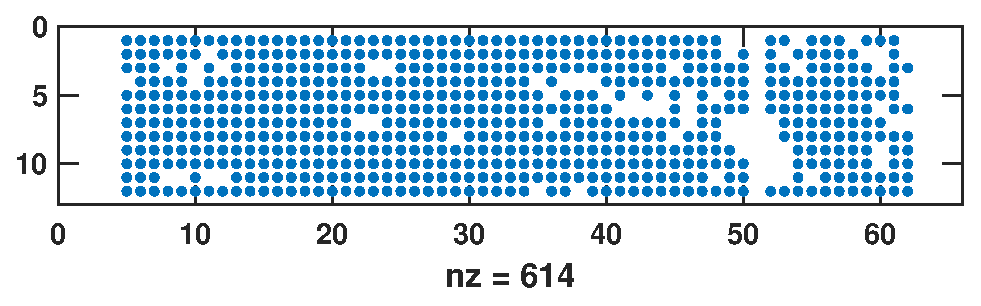
\includegraphics[width=0.43\textwidth]{figs/MH454_F_inl.eps} \\
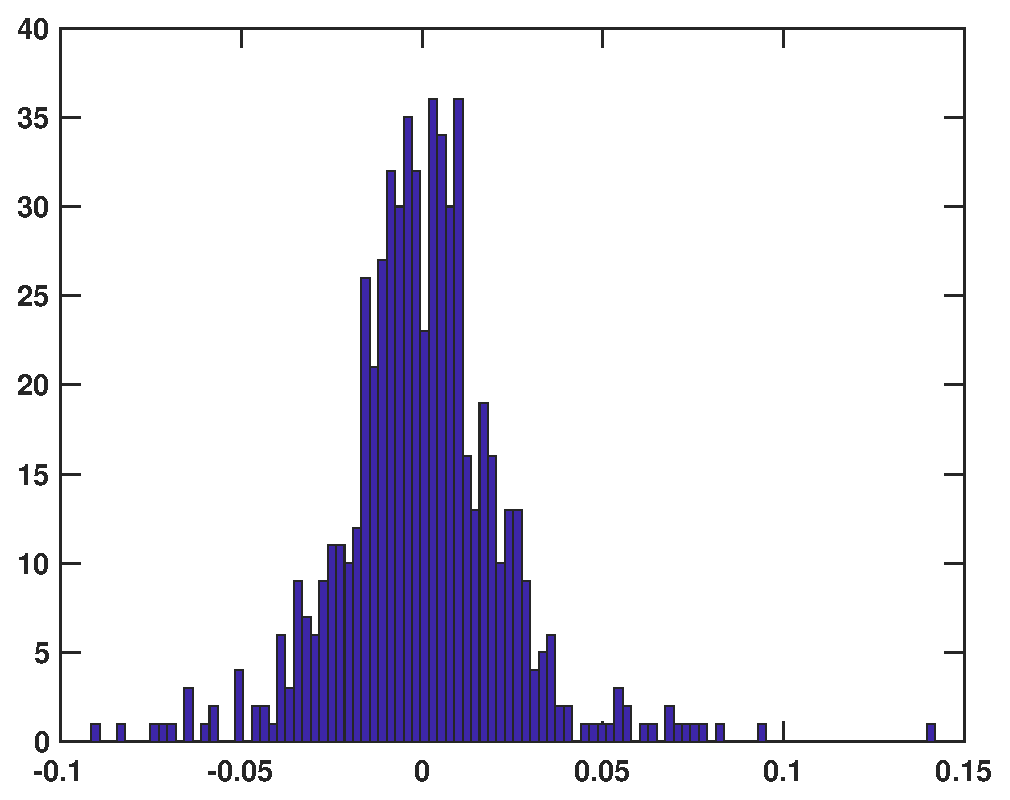
\includegraphics[width=0.21\textwidth]{figs/MH454_F_res.eps} 
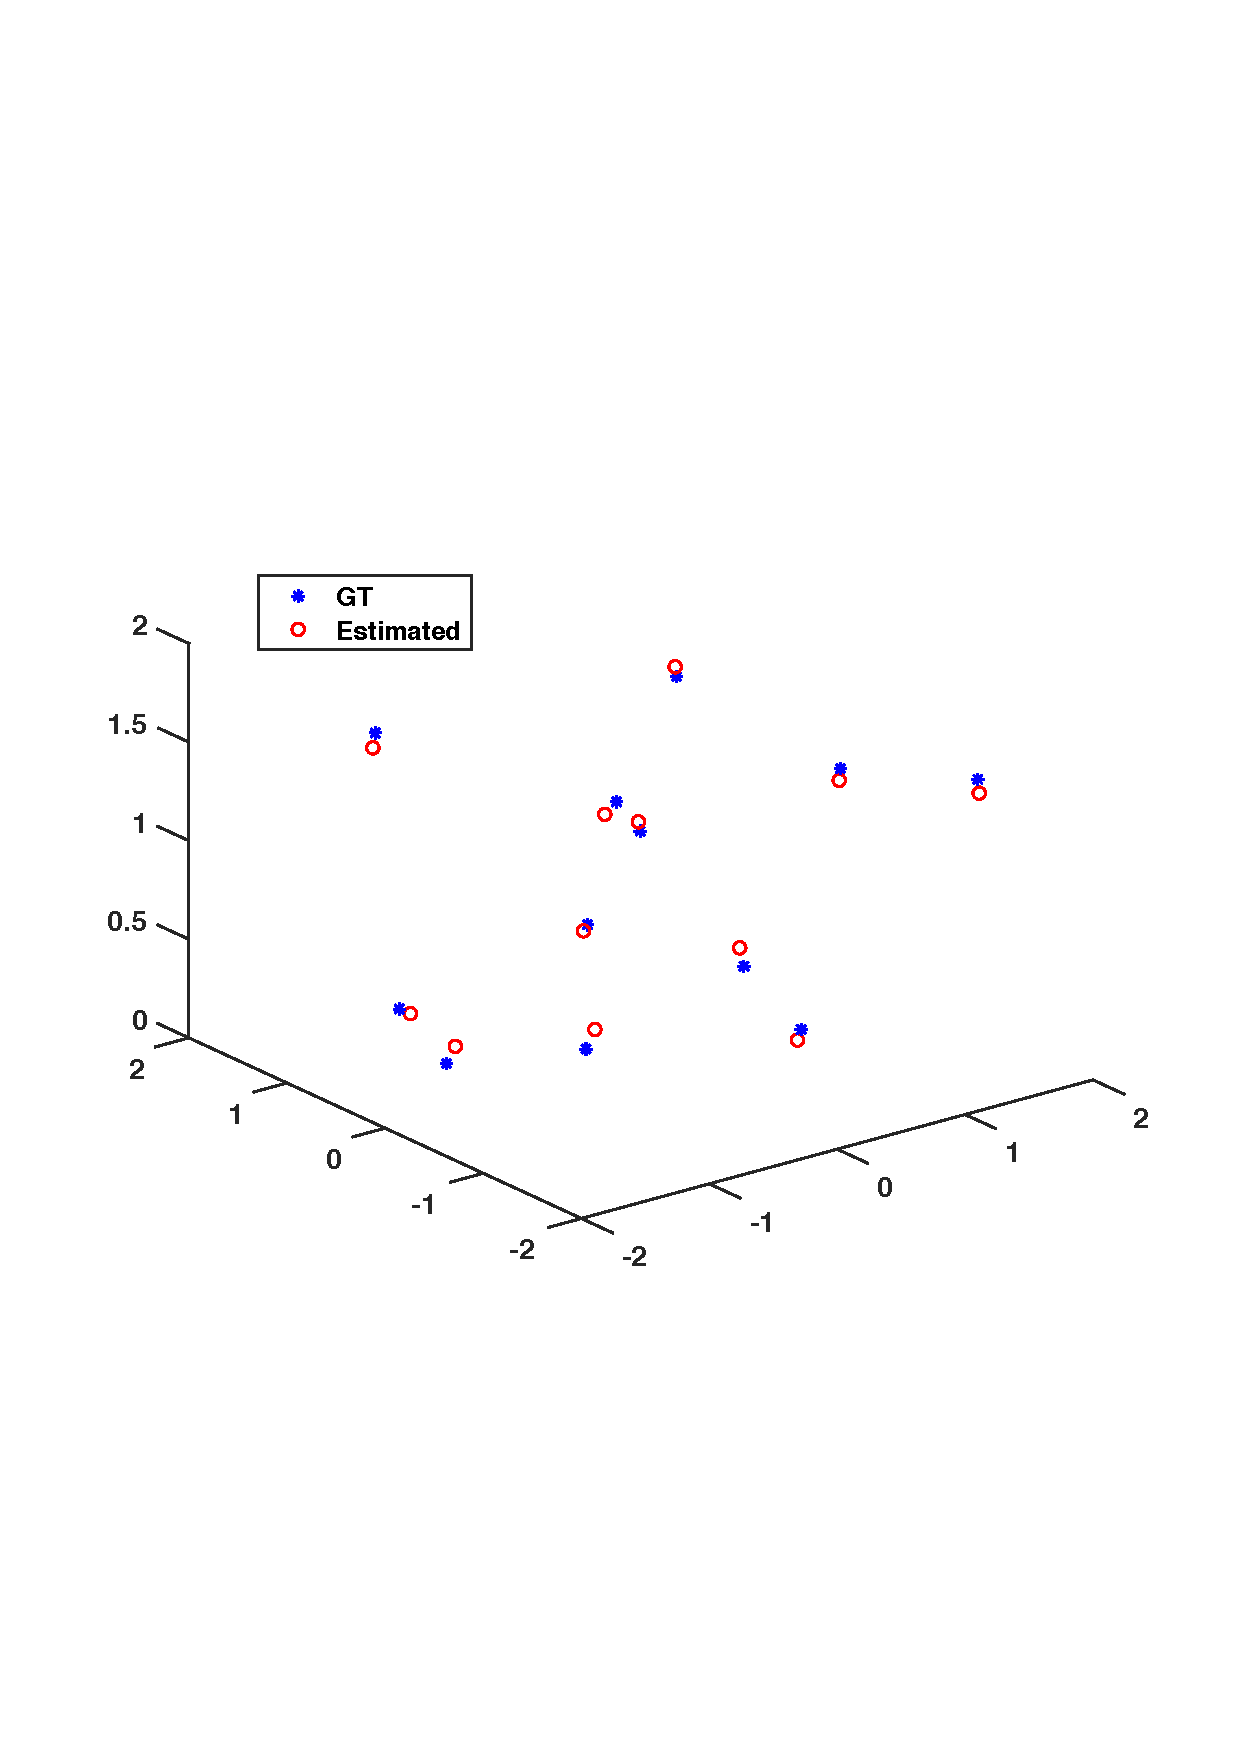
\includegraphics[width=0.26\textwidth]{figs/MH454_F_fig_new.pdf} 
\end{tabular}
\caption{For the office experiment the figure shows  detected inliers $\Win$ (top),  inlier residual histogram (bottom left), and  estimated and ground truth microphone positions (bottom right).}
\label{f_454H}
\end{figure}


\begin{figure}
\begin{tabular}{c}
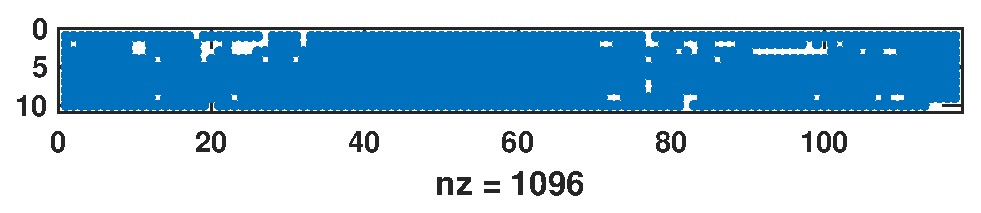
\includegraphics[width=0.43\textwidth]{figs/bat_20180710_inl.eps} \\
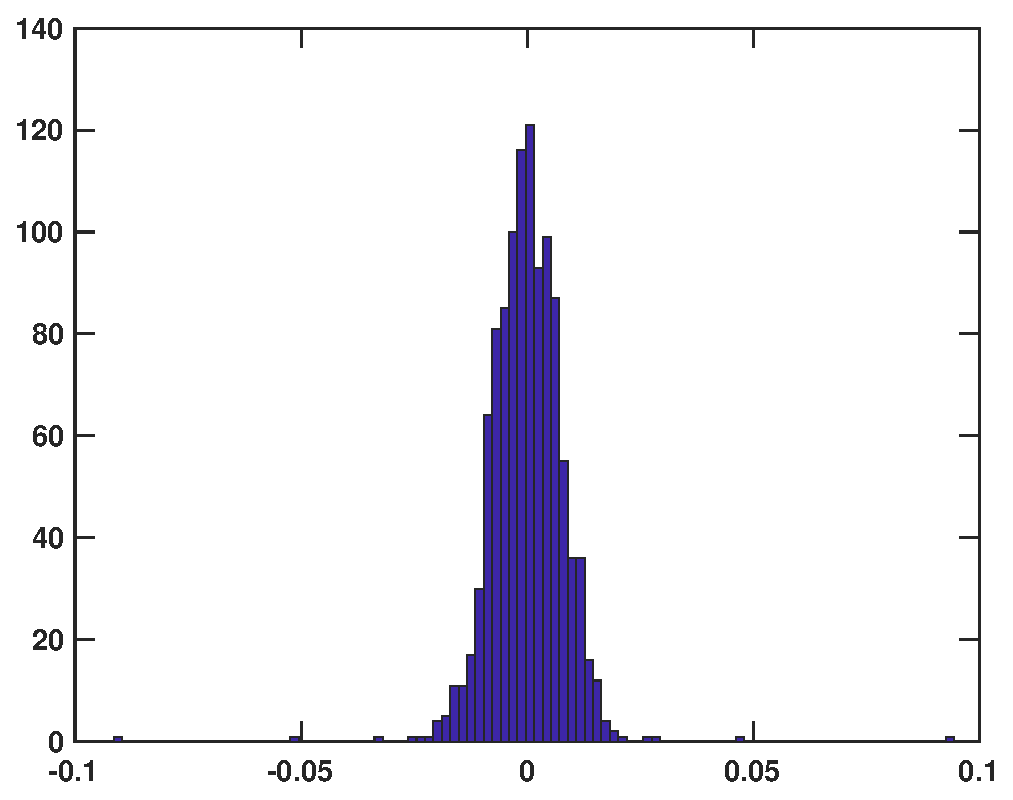
\includegraphics[width=0.24\textwidth]{figs/bat_20180710_res.eps} 
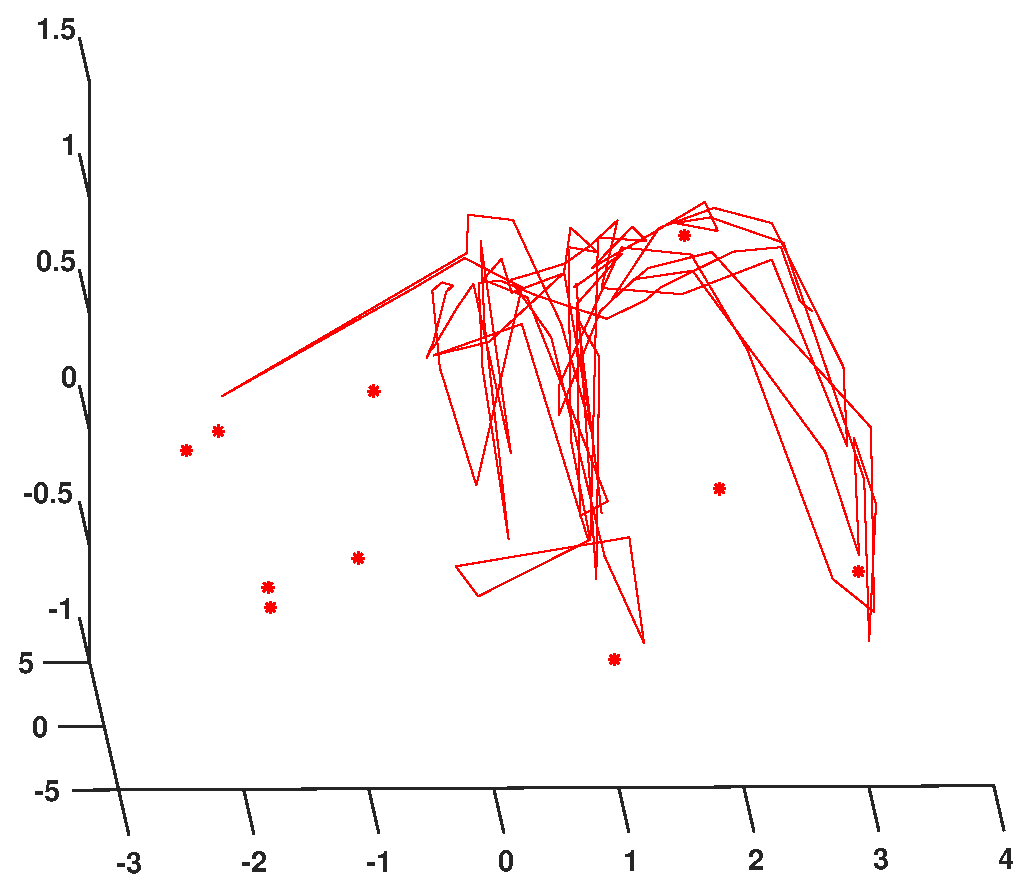
\includegraphics[width=0.23\textwidth]{figs/bat_20180710_fig.eps} \\
\end{tabular}
\caption{For the cave experiment the figure shows detected inliers $\Win$ (top), inlier residual histogram (bottom left) and  estimated microphone and sound source positions, red dots and line respectively (bottom right).}
\label{f_bat}
\end{figure}

\vspace{-5pt}
\section{Conclusions}
\label{sec:exp}
\vspace{-5pt}
In this paper, a novel method has been constructed to efficiently solve a TDOA problem with a constant offset. This has been verified using simulated data to test the solver and real experimental data to test our algorithms in realistic scenarios.

Looking at Figure~\ref{fig:f_hist} and Table~\ref{Tabletime}, it can be seen that the calculation of the offsets and the calculation of the relaxed form $\theta_2$ are very fast solvers without loss in numerical accuracy. The advantage of this is that when using a RANSAC approach, the iterations are performed quickly, giving a good initial estimate in which to optimize over, which is important in highly
non-linear systems such as this.

Looking at the results from the office experiment, Figure~\ref{f_454H}, we can see that the calculated microphone positions are accurate and the residuals are small, mostly in the range $\pm 0.04~m$. Further to this our inlier set appears to be accurate. The first and last few columns (corresponding to sound emissions) are not used in our initialisation. This is correct because the recording started before the chirps were sounded and ended after, so the chirp detection algorithm falsely determined that they were also chirps but our method decided that the data in those regions do not fit the model. A comparison of the calculated microphone positions were made to a solution from a Full TDOA system, \cite{kuang2013stratified}, which produced similar results and very similar residuals. This provided a sanity check that the chirp detection was working correctly and that from this dataset a better solution could not be found.

For the cave experiment, similar conclusions can be made, since the residuals are very low, we can conclude that we have an accurate model. This gives a real life example of how algorithms such as the one proposed can be used.

For future work, the study of the number of inliers could be of use. At the moment our algorithm may not extend to more rows and columns if the initial solution is poor, perturbing our final solution. Perhaps a method which could adapt the initial selection in order to give a required amount of inliers could be more advantageous.





\vfill\pagebreak

%\section{REFERENCES}
%\label{sec:refs}

% References should be produced using the bibtex program from suitable
% BiBTeX files (here: strings, refs, manuals). The IEEEbib.bst bibliography
% style file from IEEE produces unsorted bibliography list.
% -------------------------------------------------------------------------
\bibliographystyle{IEEEbib}
%\bibliographystyle{harvard}
\bibliography{main}

\end{document}
